\chapter{\ifproject%
\ifenglish Project Structure and Methodology\else โครงสร้างและขั้นตอนการทำงาน\fi
\else%
\ifenglish Project Structure\else โครงสร้างของโครงงาน\fi
\fi
}

ในบทนี้ จะกล่าวถึงหลักการ,  การนําทฤษฎีที่เกี่ยวข้องมาประยุกต์ใช้  และการออกแบบของระบบ


\makeatletter

% \renewcommand\section{\@startsection {section}{1}{\z@}%
%                                    {13.5ex \@plus -1ex \@minus -.2ex}%
%                                    {2.3ex \@plus.2ex}%
%                                    {\normalfont\large\bfseries}}

\makeatother
%\vspace{2ex}
% \titleformat{\section}{\normalfont\bfseries}{\thesection}{1em}{}
% \titlespacing*{\section}{0pt}{10ex}{0pt}
\section{โครงสร้างของระบบ}
% \ref{fig:Overall project structure}

% app -> streaming -> ci classify -> results -> Display -> add to cart -> payment -> order
Application โทรศัพท์มือถือ จะสามารถ classify สินค้าได้โดย application จะการถ่ายภาพของสินค้า และทำการ streaming ผ่าน WebSocket 
ไปยัง server ที่มี Computational Intelligence ทำหน้าที่ classification ข้อมูลที่ได้รับเข้ามา  และตอบกับข้อมูลชนิดสินค้าและราคา กลับไปยัง application
ผู้ใช้งาน application จะสามารถเพิ่มสินค้าที่ application ถ่าย ไปยังตะกร้าสินค้า และสามารถ กดจ่ายเงินซื้อสินค้าได้

 โดยร้านค้าจะการ บันทึกประวัตืการซื้อขาย ของสินค้าภายในร้านทำให้สามารถจัดการ จำนวนของสินค้าภายในร้าน โครงสร้างของระบบ CapSnap จะเป็นดังรูป \ref{fig:Overall project structure}



\begin{figure}[h]
  \begin{center}
  
  \vspace{0.5cm}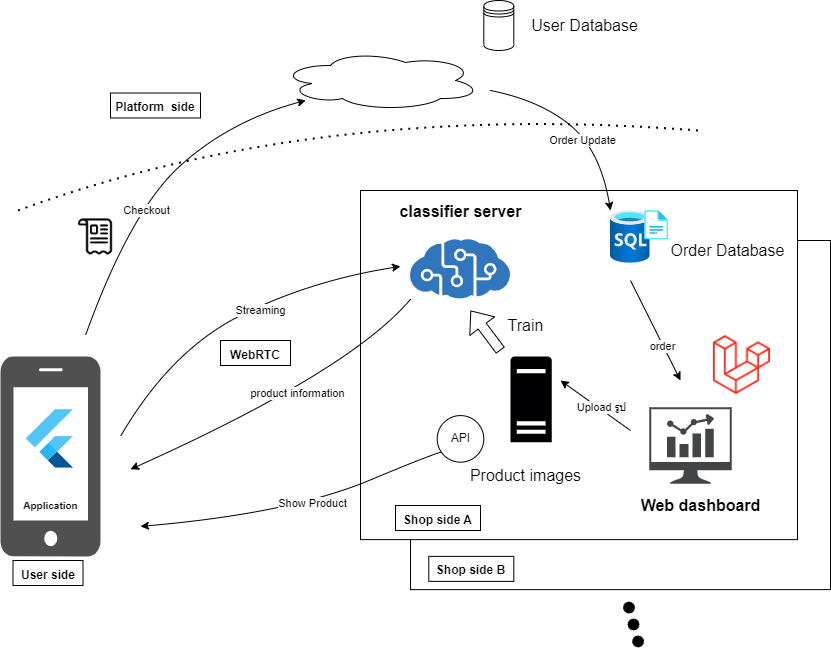
\includegraphics[scale=0.3]{pic/overall_2.png}
  \end{center}
  
  \caption[Overall project structure]{Overall project structure}
  \label{fig:Overall project structure}
  \end{figure}

  \newpage
  \subsection{แผนภาพกระแสข้อมูล (Data Flow Diagram)}
 จากขั้นตอนการทำงานของระบบ  และการ Communication ของ application และ server ของร้านค้า  
 จะมีโครงสร้างของ Data Flow Diagram ดังรูป \ref{fig:Data Flow Diagram}
\begin{figure}[h]
  \begin{center}
   
  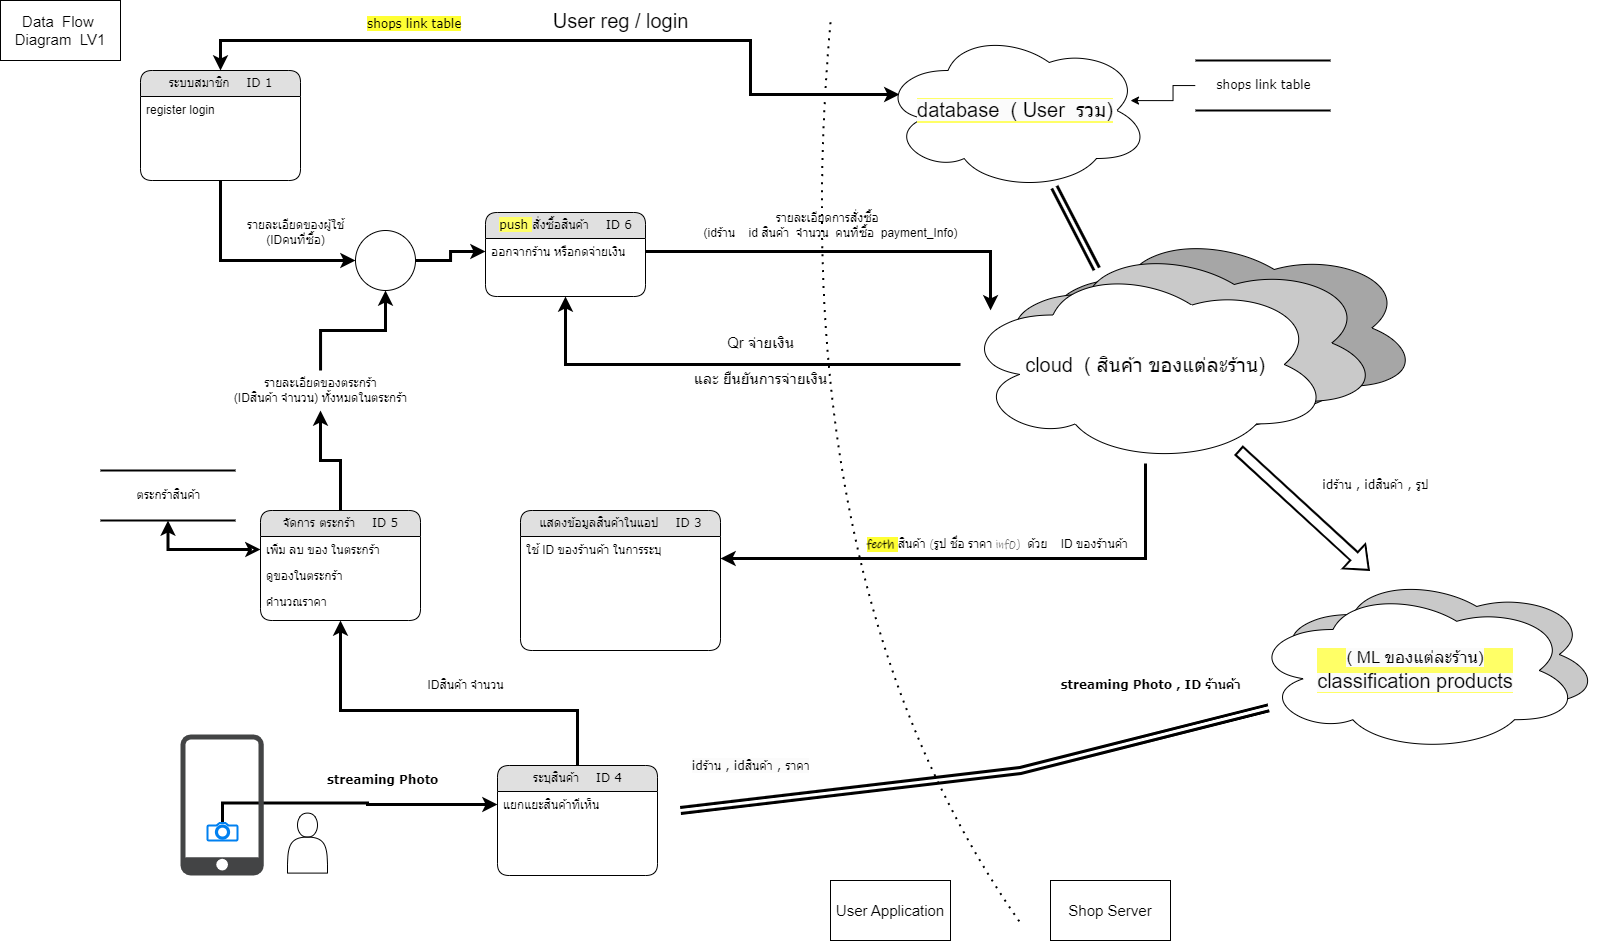
\includegraphics[scale=0.25]{pic/dataflow-lv0.png}
  \end{center}
  
  \caption[Data Flow Diagram]{Data Flow Diagram}
  \label{fig:Data Flow Diagram}
  \end{figure}

 

\section{เตรียมชุดข้อมูลฝึกสอน}
ข้อมูลที่ใช้ในการ train model ใช้รูปภาพจากสินค้าสินค้าจากห้อง 422  ทำการจัดเก็บข้อมูลรูปภาพ โดยใช้กล้องมือถือ
ในการถ่ายภาพโดยสินค้า 1 class (ชนิด) ทำการถ่ายภาพ 8 รูป ในมุมที่แตกต่างกัน  
โดยโมเดลในโครงงานนี้จะใช้สินค้าทั้งหมด 51 class และเพิ่มอีก 1 class สำหรับพื้นหลัง (background class)
รวมเป็น 52 class
จัดเก็บใน Google Drive ดังรูป  \ref{fig:Google Drive} โดยทำการแยก รูปภาพตามหมวดหมู่ และทำการดึงข้อมูลมา train ผ่าน Google Colab 
\begin{figure}[h]
  \begin{center}
   
  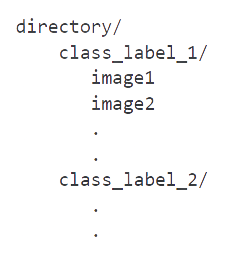
\includegraphics[scale=0.4]{pic/st.png}
  \end{center}
  
  \caption[Google Drive]{Google Drive}
  \label{fig:Google Drive}
  \end{figure}

\section{K-Fold Cross Validation}
ข้อมูลที่ใช้ในการ train model ใช้รูปภาพจากสินค้าสินค้าจากห้อง 422  ทำการจัดเก็บข้อมูลรูปภาพ โดยใช้กล้องมือถือ ในการถ่ายภาพ ในมุมต่างๆ
ของตัวสินค้า จำนวน class ละ 8 รูป โดยโมเดลในโครงงานนี้จะใช้สินค้าทั้งหมด 51 class , 1 class สำหรับพื้นหลัง (background class)
จัดเก็บใน Google Drive โดยทำการแยก รูปภาพตามหมวดหมู่ และทำการดึงข้อมูลมา train ผ่าน Google Colab
% \begin{figure}[h]
%   \begin{center}
   
%   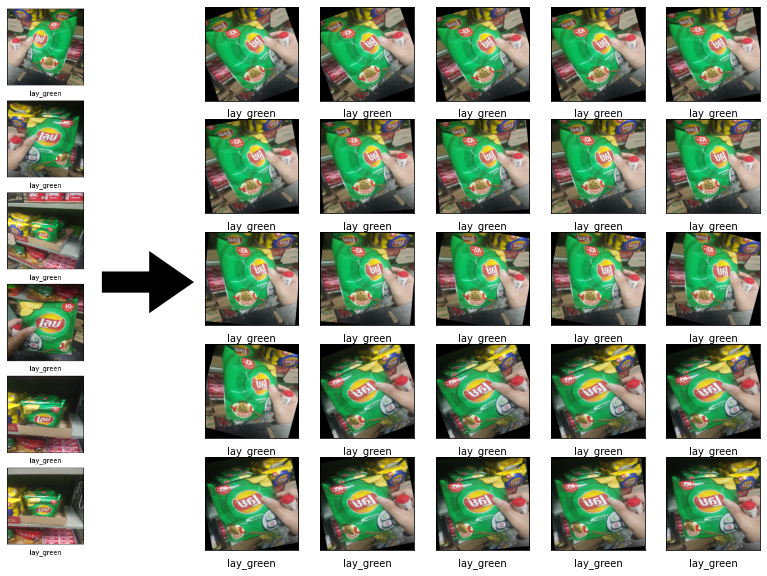
\includegraphics[scale=0.4]{pic/lay_genmore.png}
%   \end{center}
  
%   \caption[Dataset generator]{Dataset generator}
%   \label{fig:Dataset generator}
%   \end{figure}

\section{Data augmentation การเพิ่ม traing data}
เพื่อให้มี train dataset ในจำนวนมาก  
โดยในแต่ละ 1 รูปภาพที่ถ่าย จะแปลงเป็นรูปภาพ RGB ขนาด 224x224 pixel ซึ่งเป็นข้อมูล Array ขนาด 224x224x3 ในแต่ละรูป
และ   นำไปหมุนและกลับด้าน ด้วยมุม -20,-15,-10,-5,0,5,10,15,20 องศา
โดย 1 รูปภาพผ่านการ generate datasets จะกลายเป็น 18 รูปภาพซึ่งมีความแตกต่างกันเล็กน้อย ตามรูป \ref{fig:Dataset generator}

\begin{figure}[h]
  \begin{center}
   
  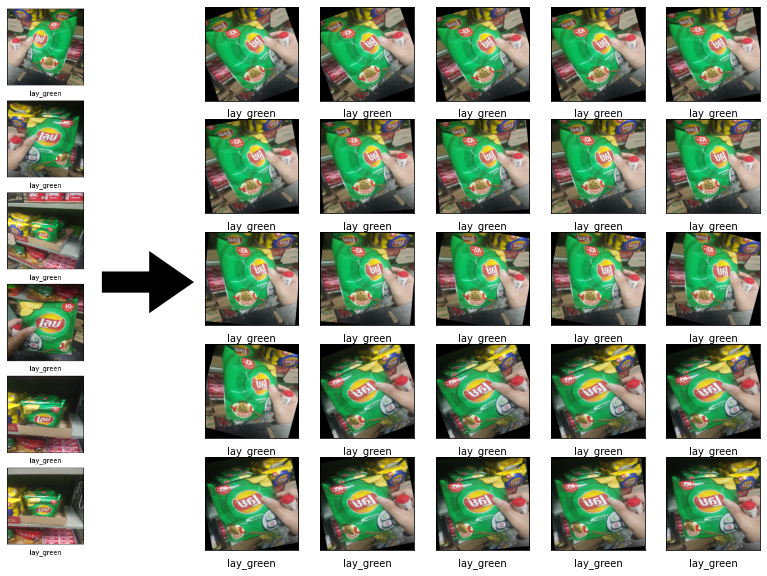
\includegraphics[scale=0.4]{pic/lay_genmore.png}
  \end{center}
  
  \caption[Dataset generator]{Dataset generator}
  \label{fig:Dataset generator}
  \end{figure}

  \newpage
\subsection{Model Architecture}
โดยโมเดลในโครงงานนี้จะใช้ Xception pre-trained ซึ่งเป็น Convolutional Neural Network ซึ่งมีความลึก 71 layers.
เป็นโมเดลที่ผ่านการจากรูปภาพต่าง ๆ มากกว่าล้านรูปภาพจาก ImageNet database .
ซึ่งจะมีโครงสร้างดังรูป


\begin{center}
  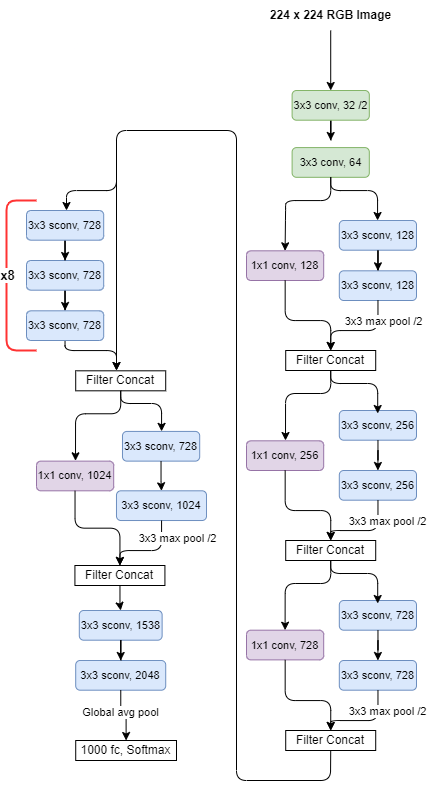
\includegraphics[scale=0.35]{pic/x_1.png}\cite{Xception}
  \end{center}


โดยการนำ Xception model มาใช้ในการแยกคุณลักษณะเด่นของรูปภาพ  และ สร้างโมเดลมาต่อท้ายเพื่อ 
เรียนรู้ลักษณะเด่นจากที่ Xception ทำการแยกออกมาได้
 
  
% transfer learning - Xceptionโดย pre-train 'Xception' model 
 
 

\begin{center}
  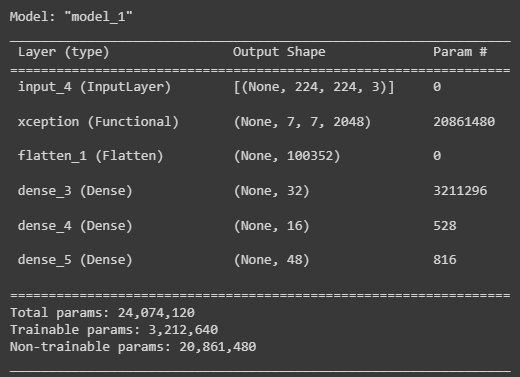
\includegraphics[scale=0.45]{pic/model.png}
\end{center}
  
ซึ่ง model ที่จะใช้ก็จะเป็น Xception model ที่รับ Input ขนาด 224 x 224 x 3 ตามขนาดรูปภาพ 224 pixel และตาม layer RGB

โดย Xception เป็น model ตั้งต้นที่่ผ่าน pre train model จะทำหน้าที่เป็น feature exercitation ลักษณะเด่นของรูปภาพ
โดย Xception จะถูก lock ค่าของ weight เอาไว้เพื่อไม่ไห้ค่าของ weight ที่ได้เรียนรู้ข้อมูลมาจาก ImageNet หายไป  ซึ่งมีทั้ง weight ทั้งหมด 20 ล้าน paramiter

 และนำ layer มาต่อท้าย model ด้วย fully connected node ที่เรียกว่า Dense layer จำนวน 32 node และ 16 node และ 
layer สุดท้าย ซึ่งมีขนาดเท่ากับจำนวน class ของสินค้า ซึ่งทำหน้าที่เป็น classifier
โดย Dense layer ซึ่งเชื่อมกันแบบ fully connected ที่สามารถ เรียนรู้และปรับค่าของ weight ได้
ในโครงสร้างทดสอบนี้จะมี weight ที่่สามารถเรียนรู้หรือ เปลี่ยนแปลงได้ 3 ล้าน paramiter
   

\section{classification products}
จากรูปภาพใน 52 class ผ่านการ generate datasets จะมี dataset ทั้งหมด 4432 sample
 ทำการแบ่งเป็น train 3546 sample และ  886 sample สำหรับการ evaluate 
โดยจาก train 3546 แบ่ง 50\% สำหรับการ validation ในระหว่างการ train model

\par ผลลัพธ์ จากการ train \& validation ด้วย 3546 sample เป็นจำนวน 200 Epoch

ตัวอย่าง ผลการทดลองของการ validation ด้วย 3546 sample
\begin{figure}[h]
  \begin{center}
  
  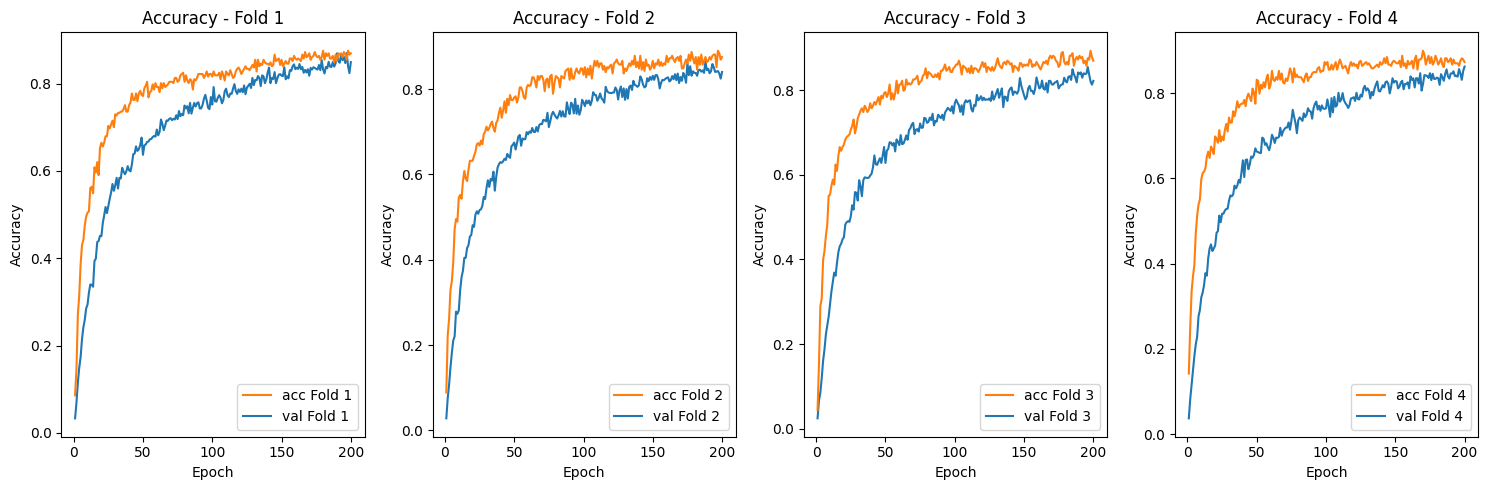
\includegraphics[scale=0.4]{pic/train_fold.png}
  \end{center}
  
  \caption[Train fold]{Train fold}
  \label{fig:Train fold}
  \end{figure}

  % โดยเมื่อนำ evaluate มาหา cross_entropy 0.23343226313591003, 0.944695234298706 accuracy

  และทำการเลือก model ที่มีค่า Validation Score สูงสุดจากใน 4 model  
  เพื่อนำไปทำการ Blind Test 
  โดยได้นำ model ใน  Fold 4   มาทำการ
  Evaluate (Blind Test)
  \begin{align}
    \text{cross\_entropy} &= 1.175 \\
    \text{accuracy} &= 0.72
  \end{align}
 

  (Blind Test)

  \begin{figure}[h]
    \begin{center}
    
    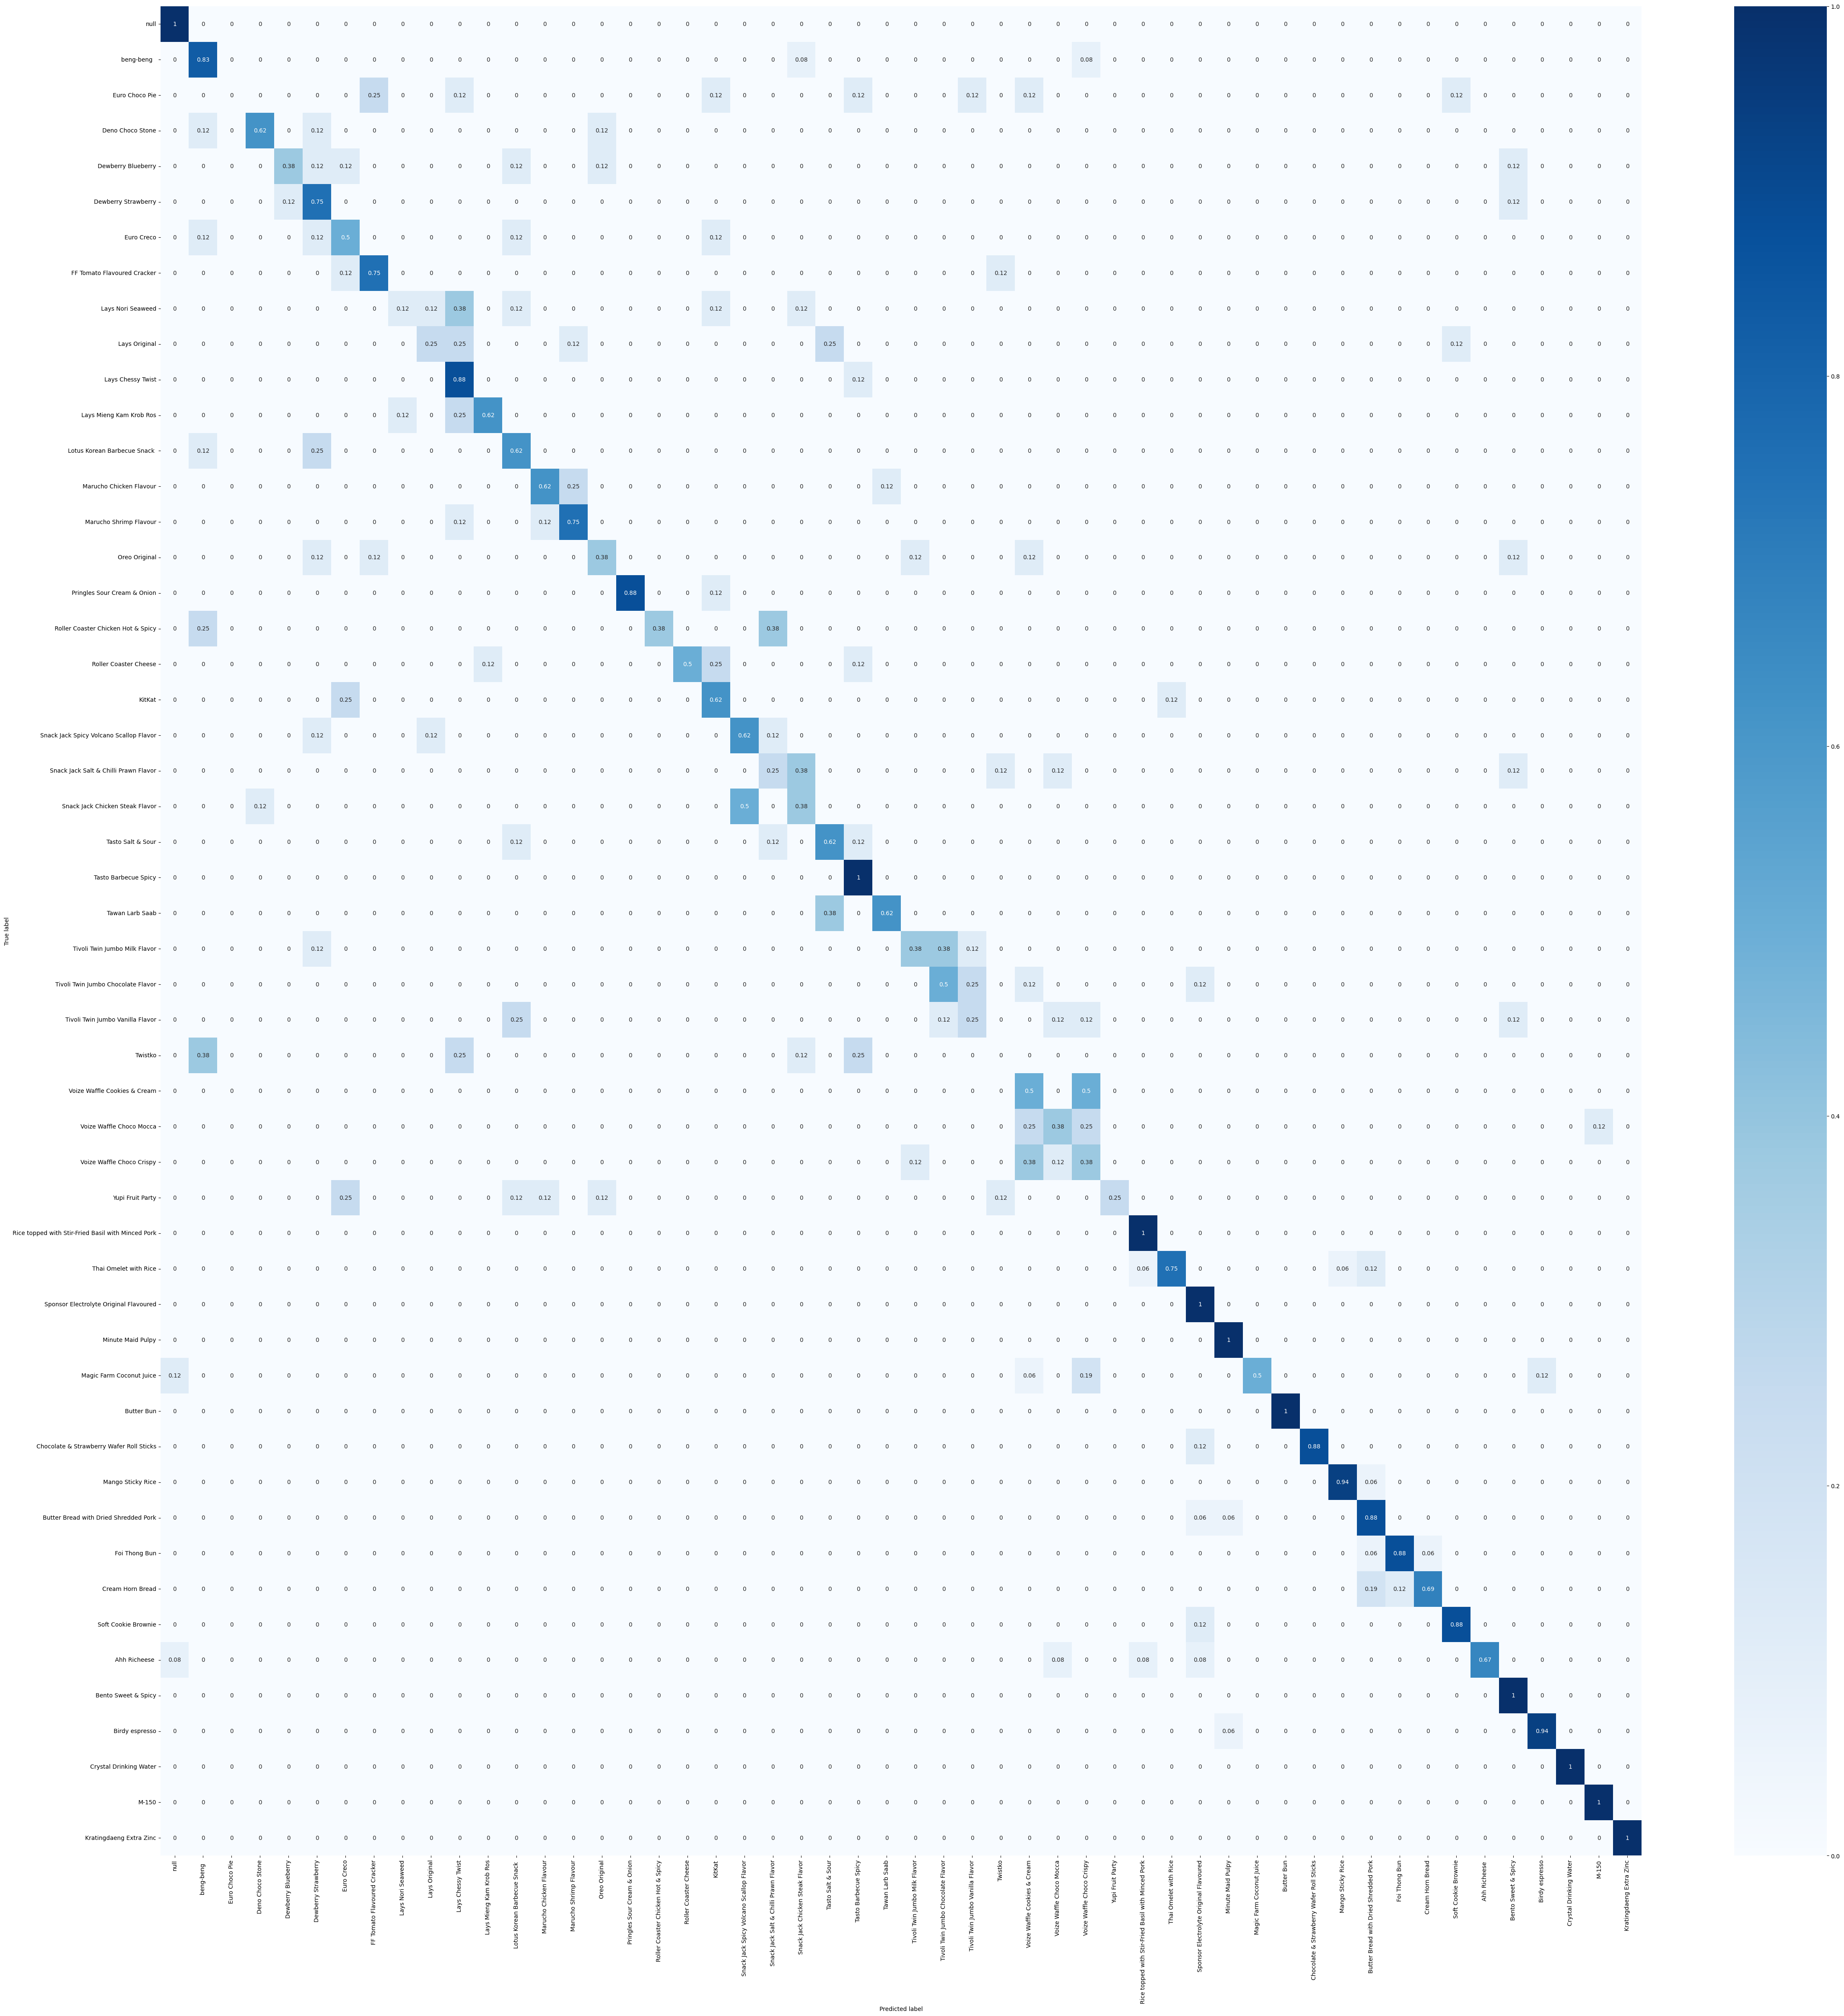
\includegraphics[scale=0.12]{pic/blind_pic_4_ccm.png}
    \end{center}
    
    \caption[Confusion matrix]{Confusion matrix}
    \label{fig:Confusion matrix}
    \end{figure}
   สำหรับเป็น service ในการ classify products ของ application ผ่าน aiortc  และเว็บ WebSocket

 
 
\newpage

\section{การพัฒนา Mobile Application}
ใช้ Flutter ในการสร้าง Mobile Application ในส่วนของผู้ใช้โดยใช้ service ของ WebSocket ติดต่อกับ Classification server ที่ได้ทำการฝึกสอนไว้แล้ว
โดยจะแอพลิเคชันจะมีฟังก์ชันที่ทำการสตรีมมิ่งภาพสินค้าที่ลูกค้าถ่ายผ่าน WebSocket ไปยัง server ของทางร้านซึ่งมี Model classifier อยู่
จากนั้น Server ของทางร้านจะ Classifiy ว่าเป็นสินค้าชนิดใด และตอบกลับมายังแอพลิเคชันเพื่อแสดงผลให้กับผู้ใช้งาน
\subsection{Requirement Specification}  

\begin{enumerate}
  \item ผู้คนทั่วไปสามารถลงทะเบียนเข้าใช้งานได้ผ่าน SSO อีเมล์ และหมายเลขโทรศัพท์มือถือ
  \item สามารถเชื่อมต่อกับข้อมูลร้านค้าได้ผ่านการแสกนคิวอาร์โค้ดเข้าใช้งานร้านค้า
  \item สามารถใช้กล้องโทรศัพท์มือถือแสกนสินค้าเพื่อสตรีมภาพ Classification server เพื่อทำการดึงข้อมูลสินค้าจาก Server ของร้านค้ามาแสดงผลบนแอพลิเคชัน
  \item สามารถเพิ่มหรือลดสินค้าในตะกร้าได้
  \item สามารถทำการชำระเงินได้ผ่าน Payment gateway ในตัวแอพลิเคชัน
  \item สามารถ Checkout จากร้านค้าผ่านการแสกนคิวอาร์โค้ดออกจากร้านค้า
 
\end{enumerate}


\section{การเตรียมฐานข้อมูล}
ในการเก็บฐานข้อมูลจะแบ่งเป็นฐานข้อมูลสองตัว โดยใช้ Supabase 
ในการสร้างโครงการ และจัดฐานข้อมูลทั้งหมดแบบ SQL ได้แก่ 
\subsection{ฐานข้อมูลของระบบ}
สำหรับเก็บข้อมูลร้านค้าที่เข้าร่วม และประวัติการซื้อสินค้าของผู้ใช้งานแอพลิเคชันมือถือ ซึ่งมี Database schema ดังนี้ 
\begin{figure}[h]
\begin{center}
 
  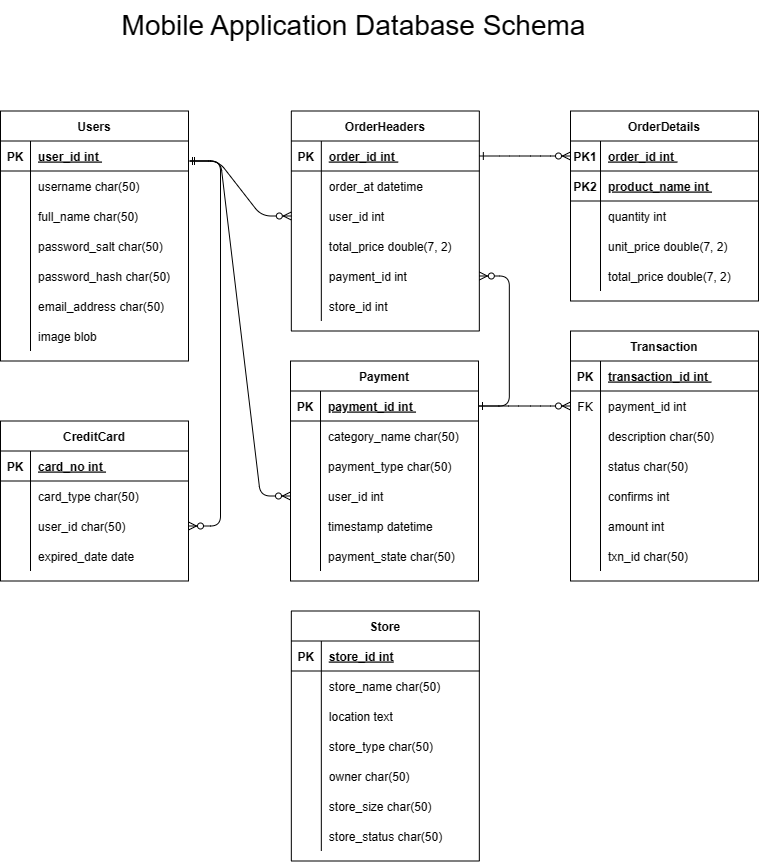
\includegraphics[scale=0.3]{pic/datamobile.png}
  \end{center}
  
  \caption[Mobile Application Database Schema]{Mobile Application Database Schema}
  \label{fig:Mobile Application Database Schema}
  \end{figure}


  
\subsection{ฐานข้อมูลในแต่ละร้านค้า}
สำหรับเก็บข้อมูลสินค้า และประวัติยอดขายของร้านค้า โดยร้านค้าแต่ละร้านจะมีฐานข้อมูลเป็นของตนเองเพื่อใช้งานกับ Server ของร้านนั้น ๆ
 โดยตรง ซึ่งจะมี Database schema ดังนี้ 

 \begin{figure}[h]
  \begin{center}
 
    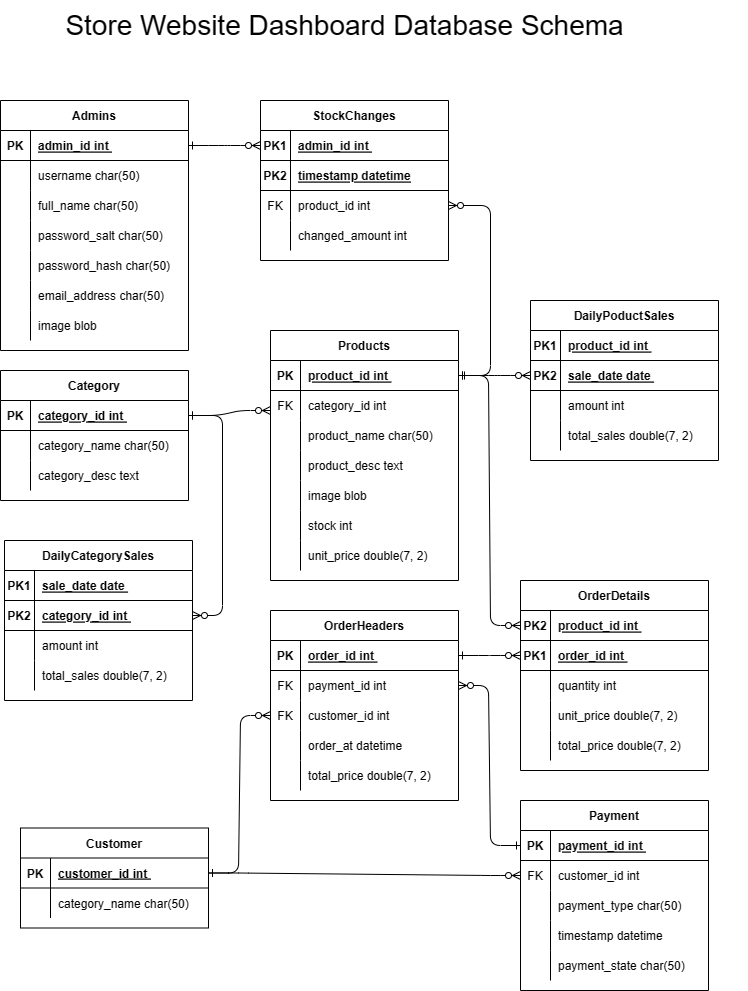
\includegraphics[scale=0.3]{pic/dataweb.png}
    \end{center}
    
    \caption[Store Website Dashboard Database Schema]{Store Website Dashboard Database Schema}
    \label{fig:Store Website Dashboard Database Schema}
    \end{figure}
  
\section{การพัฒนา Website Dashboard }


ออกแบบ UI/UX ของ Wedsite Dashboard และ Mobile Application ด้วย Figma
หลังจากการออกแบบ และจัดการตั้งค่าฐานข้อมูลเสร็จแล้ว
 ก็จะพัฒนาในส่วนของเว็บไซต์ทางฝั่งร้านค้าโดยใช้ Supabase ในการโฮสติ้งเว็บไซต์ 
 และเชื่อมต่อกับฐานข้อมูลที่ได้ตั้งค่าไว้ โดยใช้ Flask framework 
 ในการจัดการ API และ Python ในการจัดการระบบ Backend ของเว็บไซต์โดยใช้ SQLAlchemy
  ในการดึงข้อมูลจากฐานข้อมูล Requirement Specification ดังนี้

  \begin{enumerate}
    \item สามารถเข้าใช้งานได้ผ่านการยืนยันตัวตนเป็น Administers เท่านั้น โดยสามารถมีได้ 1-5 คน
    \item สามารถดูคลังสินค้า และแก้ไขข้อมูลสินค้าในแต่ละชนิดได้แบบเรียลไทม์
    \item สามารถดูสถิติยอดขายสินค้าได้ทั้งแบบรายวัน รายเดือน และรายปี โดยแบ่งได้ 2 แบบ คือตามชนิดสินค้า และประเภทสินค้า
    \item สามารถดูประวัติการขายตามออเดอร์ของลูกค้าแต่ละคนได้ และดูข้อมูลของแต่ละออร์เดอร์ได้
\end{enumerate}



 

\section{การทดสอบการทำงานของซอร์ฟแวร์}
การทดสอบการทำงานของระบบ สามารถแบ่งเป็นขั้นตอนดังนี้
\subsection{Unit testing}
การทดสอบความถูกต้องของการทำงานในแต่ละฟังก์ชันหลักของระบบแยกกัน โดยยังไม่รวมแต่ละ Component เข้าด้วยกัน ซึ่งได้แก่
\begin{enumerate}
  \item Classification system
  \item Website dashboard
  \item Mobile Application
\end{enumerate}

\subsection{Integration testing}
การทดสอบการทำงานเมื่อรวมระบบย่อยทั้งหมดเข้าด้วยกัน โดยหลัก ๆ
 จะทดสอบในเรื่อง API ว่ามีการรับส่งข้อมูลดุถูกต้องหรือไม่ และทำงานโดยรวมได้ถูกต้องทั้งหมดหรือไม่
\subsection{System testing}
การทดสอบระบบซึ่งแต่ละโมดูลข้างต้นจะถูกรวม และทดสอบเป็นกลุ่ม 
เพื่อประเมินความสอดคล้องของระบบว่าทำงานได้ตามที่กำหนดไว้หรือไม่
\subsection{Acceptance testing}
การทดสอบระบบโดยดูภาพรวมของการทำงาน ว่ามีการตอบสนองความต้องการของผู้ใช้ทั้งในส่วนของฟังก์ชันการทำงาน 
และประสิทธิภาพการทำงาน ว่าสอดคล้องกับลักษณะของความต้องการของซอฟต์แวร์หรือไม่ 
โดยใช้การทดสอบแบบ Functional testing (Black box testing)
 
  

% \subsection{The Black Kitten}
  % One thing was certain, that the WHITE kitten had had nothing to
% do with it:---it was the black kitten's fault entirely



% ~\cite{aiw}. 




%  For the
% white kitten had been having its face washed by the old cat for
% the last quarter of an hour (and bearing it pretty well,
% considering); so you see that it COULDN'T have had any hand in
% the mischief.

%   The way Dinah washed her children's faces was this:  first she
% held the poor thing down by its ear with one paw, and then with
% the other paw she rubbed its face all over, the wrong way,
% beginning at the nose:  and just now, as I said, she was hard at
% work on the white kitten, which was lying quite still and trying
% to purr---no doubt feeling that it was all meant for its good.

%   But the black kitten had been finished with earlier in the
% afternoon, and so, while Alice was sitting curled up in a corner
% of the great arm-chair, half talking to herself and half asleep,
% the kitten had been having a grand game of romps with the ball of
% worsted Alice had been trying to wind up, and had been rolling it
% up and down till it had all come undone again; and there it was,
% spread over the hearth-rug, all knots and tangles, with the
% kitten running after its own tail in the middle.

% \subsection{The Reproach}

  